
\section{講義概要}

\begin{frame}
\frametitle{接平面}

二変数関数$f(x,y)=x^2+3y^2$のグラフの点$(1,2,13)$における接平面を求める. 
$$
f_x(x,y)=2x=2, \ \ \ f_y(x,y)=6y=12
$$
より, $f(x,y)$は$C^1$級であるから, 接平面の方程式は
$$
z=13+2(x-1)+12(y-2)
$$
で与えられる. 整理すれば
$$
z=2x+12y-13. 
$$

\end{frame}


%%%%%%%%%%%%%%%%%%%%%%%%%%%%%%%%%%%%%%%%%%%%%%%%%%%%%%%%%%%%%%%%%%%%%%%%%%%%%%%%%%%%%%%
%%%%%%%%%%%%%%%%%%%%%%%%%%%%%%%%%%%%%%%%%%%%%%%%%%%%%%%%%%%%%%%%%%%%%%%%%%%%%%%%%%%%%%%


\begin{frame}
\frametitle{極値と停留点}

以下では, 二変数関数$f(x,y)$は$C^2$級であるとする. 
$f(x,y)$の\underline{停留点}とは, $f_x(a,b) = f_y(a,b) = 0$を満たす$(a,b)$をいう. 

\begin{Thm} \label{極値->停留点}
関数$f(x,y)$が$(a,b)$で極値(極大値または極小値)を取るとき, $(a,b)$は停留点となる. 
\end{Thm}

\begin{itemize}
\item 定理\ref{極値->停留点}は, 一変数関数$f(x,b)$と$f(a,y)$が$(a,b)$で極値を取ることから従う. 
\item 停留点は極値とは限らない. 例えば, \underline{鞍点(あんてん：saddle point)}と呼ばれる, ある方向から見ると極大値, 別の方向から見ると極小値となる停留点も存在する. 
\end{itemize}

\end{frame}




%%%%%%%%%%%%%%%%%%%%%%%%%%%%%%%%%%%%%%%%%%%%%%%%%%%%%%%%%%%%%%%%%%%%%%%%%%%%%%%%%%%%%%%
%%%%%%%%%%%%%%%%%%%%%%%%%%%%%%%%%%%%%%%%%%%%%%%%%%%%%%%%%%%%%%%%%%%%%%%%%%%%%%%%%%%%%%%


\begin{frame}
\frametitle{極値問題の主定理}


\begin{Thm} \label{停留点とヘッセ行列}
関数$f(x,y)$の\underline{ヘッセ行列式}(ヘッシアン)を
$$
H(x,y)
=f_{xx}(x,y)f_{yy}(x,y)-f_{xy}(x,y)^2
$$
で定義する. 
停留点$(a,b)$に関して 
\begin{itemize}
\item $H(a,b)>0, \ f_{xx}(a,b)>0 \ \Longrightarrow$ $f(x,y)$は$(a,b)$で極小, 
\item $H(a,b)>0, \ f_{xx}(a,b)<0 \ \Longrightarrow$ $f(x,y)$は$(a,b)$で極大, 
\item $H(a,b)<0 \ \Longrightarrow$ $(a,b)$は$f(x,y)$の鞍点. 
\end{itemize}
\end{Thm}

%$H(a,b)>0$の下で, 条件$f_{xx}(a,b) \gtrless 0$は条件$f_{yy}(a,b)\gtrless 0$と同値であることに注意する. 
証明は後述。
\end{frame}



%%%%%%%%%%%%%%%%%%%%%%%%%%%%%%%%%%%%%%%%%%%%%%%%%%%%%%%%%%%%%%%%%%%%%%%%%%%%%%%%%%%%%%%
%%%%%%%%%%%%%%%%%%%%%%%%%%%%%%%%%%%%%%%%%%%%%%%%%%%%%%%%%%%%%%%%%%%%%%%%%%%%%%%%%%%%%%%


\begin{frame}
\frametitle{極値問題}

関数$f(x,y)=x^2+x^2y+y^2$の極値を調べる. まず
\begin{align*}
f_x(x,y) &= 2x+2xy=2x(1+y)=0\\ 
f_y(x,y) &= x^2+2y=0
\end{align*}
を解くことで, 停留点は
$$
(x,y)=(0,0), \ (\pm \sqrt{2},-1)
$$
だと分かる. 

\end{frame}


%%%%%%%%%%%%%%%%%%%%%%%%%%%%%%%%%%%%%%%%%%%%%%%%%%%%%%%%%%%%%%%%%%%%%%%%%%%%%%%%%%%%%%%
%%%%%%%%%%%%%%%%%%%%%%%%%%%%%%%%%%%%%%%%%%%%%%%%%%%%%%%%%%%%%%%%%%%%%%%%%%%%%%%%%%%%%%%


\begin{frame}
\frametitle{極値問題}
また2次偏導関数は
$$
f_{xx}(x,y)=2(1+y), \ \ \ f_{xy}(x,y)=2x, \ \ \ f_{yy}(x,y)=2
$$
であるから
$$
H(x,y)=2(1+y) \cdot 2 - (2x)^2=4(1+y-x^2). 
$$

\begin{itemize}
\item 点$(0,0)$に関して
\begin{align*}
H(0,0)=4>0, \ \ \ f_{xx}(0,0) = 2
\end{align*}
であるから, $f(x,y)$は $f(0,0)=0$において極小値である. 
\item 点$(\pm \sqrt{2},-1)$に関して
\begin{align*}
H(\pm \sqrt{2},-1)=-8<0
\end{align*}
であるから, $f(x,y)$は$(\pm\sqrt{2},-1)$において極値をとらない.  
\end{itemize}

\end{frame}
\begin{slide}{$f(x,y) = x^2+x^2y+y^2$のグラフ}
\begin{figure}[h]
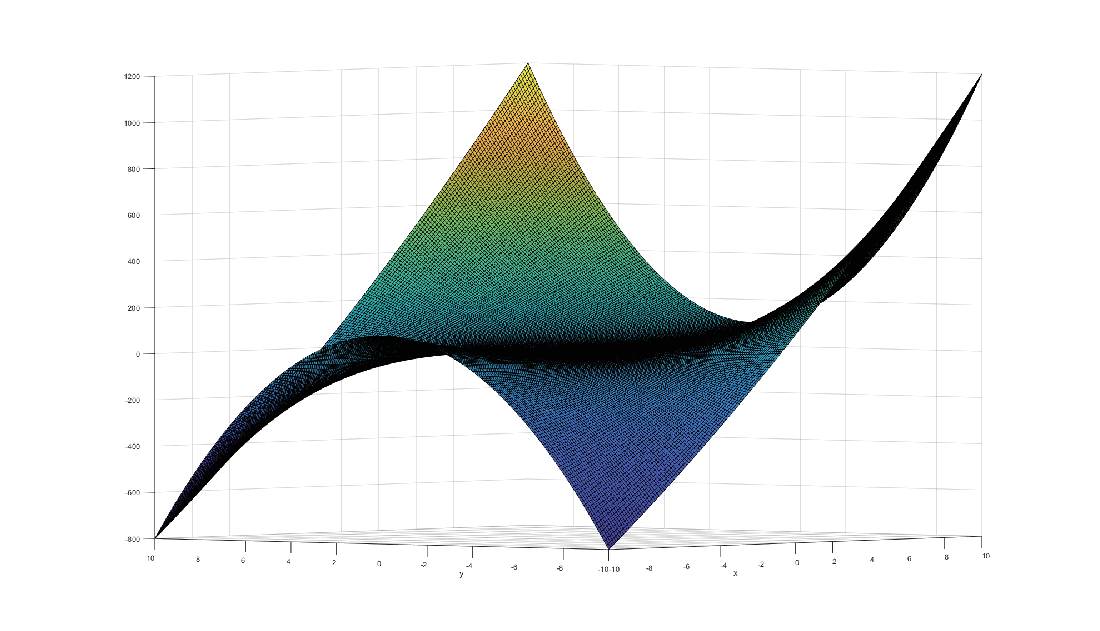
\includegraphics[width=8cm]{calculus10/twodimopt.eps}
\end{figure}
twodimopt.m参照。
\end{slide}


%%%%%%%%%%%%%%%%%%%%%%%%%%%%%%%%%%%%%%%%%%%%%%%%%%%%%%%%%%%%%%%%%%%%%%%%%%%%%%%%%%%%%%%
%%%%%%%%%%%%%%%%%%%%%%%%%%%%%%%%%%%%%%%%%%%%%%%%%%%%%%%%%%%%%%%%%%%%%%%%%%%%%%%%%%%%%%%
\begin{slide}{二変数関数のテイラー展開}

二変数のテイラー展開は以下である。
\begin{eqnarray}
f(x+h, y+k) &=& f + \left(h\frac{\partial }{\partial x} + k\frac{\partial}{\partial y}\right) f \nonumber \\ 
&+& \frac{1}{2!}\left(h\frac{\partial }{\partial x} + k\frac{\partial}{\partial y}\right) ^2 f  \nonumber \\
&+& \frac{1}{3!}\left(h\frac{\partial }{\partial x} + k\frac{\partial}{\partial y}\right) ^3f + \cdots \nonumber
\end{eqnarray}

二次まで展開すると
\begin{eqnarray}
&& f(x+h, y+k) =  f + \left(h\frac{\partial f}{\partial x} + k\frac{\partial f}{\partial y}\right)  \nonumber \\ 
&+& \frac{1}{2!}\left(h^2\frac{\partial^2 f}{\partial x^2} + 2hk\frac{\partial^2 f}{\partial x\partial y}+k^2\frac{\partial^2 f}{\partial y^2}\right)  \nonumber \\
&=& f + hf_x + kf_y + \frac{h^2}{2}f_{xx}+ hk f_{xy} + \frac{k^2}{2}f_{yy} \nonumber
\end{eqnarray}

\end{slide}

%\begin{frame}
%\frametitle{極値と停留点 (発展)}
%
%二変数関数に関しても, テイラー展開を行うことが可能で
%$C^2$級関数$f(x,y)$は停留点$(a,b)$の近傍で次の形に近似される. 
%(停留点という条件から, 一次部分は消えている.)
%\begin{align*}
%f(x,y) & \approx f(a,b)+ \frac{1}{2}f_{xx}(a,b)(x-a)^2 \\
%& \ \ \ \ \ \ +f_{xy}(a,b)(x-a)(y-b)+\frac{1}{2}f_{yy}(a,b)(y-b)^2 \\
%& =  f(a,b)+ \frac{1}{2}[x-a \ \ y-b]
%\begin{bmatrix} f_{xx}(a,b) & f_{xy}(a,b) \\ f_{yx}(a,b) & f_{yy}(a,b) \end{bmatrix}
%\begin{bmatrix} x-a \\ y-b \end{bmatrix}
%\end{align*}
%ヘッセ行列式$H(a,b)$は$\begin{bmatrix} f_{xx}(a,b) & f_{xy}(a,b) \\ f_{yx}(a,b) & f_{yy}(a,b) \end{bmatrix}$の行列式に他ならない. 
%定理\ref{停留点とヘッセ行列}は対称2次形式の分類に関係する. 
%
%\end{frame}

\begin{slide}{極大・極小の判別原理}
$x,y$の二次斉次式(せいじしき：すべての項の次数が等しい式:homogeneous polynomial)$Q(x) = Ax^2 + 2Bxy+ Cy^2$は
\begin{enumerate}
\item $AC-B^2>0, A>0$なら$(0,0)$で極小
\item $AC-B^2>0, A<0$なら$(0,0)$で極大
\item $AC-B^2<0$なら極大・極小をとらない
\end{enumerate}
証明
\begin{equation}
Q(x,y) = A\left\{\left(x + \frac{B}{A}y\right)^2 + \frac{AC-B^2}{A^2}y^2\right\}\nonumber 
\end{equation}
と変形でき$(x + \frac{B}{A}y)^2$は常に正、$AC-B^2$が正で、$A>0$の時$Q>0$（極小）, $A<0$の時$Q<0$（極大）となる。
$AC-B^2$が負の場合には、$Q$は正にも負にもなる。

これを利用し、関数$f$の二次までのテイラー展開は
\begin{equation}
f(x+h, y+k) = f(x,y) + f_x(x,y)h + f_y(x,y)k + f_{xy}(x,y)kh + \frac{f_{xx}}{2}h^2 + \frac{f_{yy}}{2}k^2 \nonumber
\end{equation}
であり、極値では$f_x(x,y)=f_y(x,y)=0$であり、斉次式を適用。
\end{slide}

%%%%%%%%%%%%%%%%%%%%%%%%%%%%%%%%%%%%%%%%%%%%%%%%%%%%%%%%%%%%%%%%%%%%%%%%%%%%%%%%%%%%%%%
%%%%%%%%%%%%%%%%%%%%%%%%%%%%%%%%%%%%%%%%%%%%%%%%%%%%%%%%%%%%%%%%%%%%%%%%%%%%%%%%%%%%%%%





%%%%%%%%%%%%%%%%%%%%%%%%%%%%%%%%%%%%%%%%%%%%%%%%%%%%%%%%%%%%%%%%%%%%%%%%%%%%%%%%%%%%%%%
%%%%%%%%%%%%%%%%%%%%%%%%%%%%%%%%%%%%%%%%%%%%%%%%%%%%%%%%%%%%%%%%%%%%%%%%%%%%%%%%%%%%%%%


%\begin{slide}{課題\#10}
%関数$f (x, y) = xy(1 - x - y) $の極値を求め、それぞれが極大か極小を判別せよ. 
%
%\end{slide}

\begin{slide}{課題\#10}
ある地域の家賃$y$万円と、部屋の広さ$x$~$\mathrm{m^2}$のデータを集めて、相場を推定する仕事を担当したとしよう。$i$番目の家賃と、部屋の広さのデータを$y_i, x_i$で表して、データが下のように$15$個集められたとする。
\begin{table}[hbt]
\centering 
%\caption{部屋の広さと家賃に関するデータ}
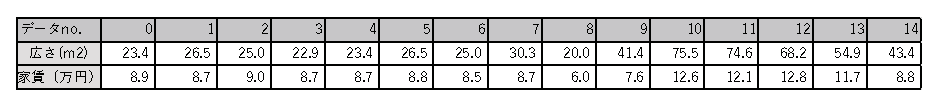
\includegraphics[width=10cm]{calculus10/renttab.eps}
\label{tab:renttab}
\end{table}
このデータを用いて部屋の広さ$x$を与えると家賃相場$y$がある定数$a, b$を用いて
\begin{equation}
y = a x + b \nonumber
\label{eq:regsimple}
\end{equation}
で計算できるようにしたい。$a,b$をデータ$(x_0, y_0), (x_1, y_1), \cdots, (x_{14}, y_{14})$を用いて、以下の損失関数$L(a,b)$を最小にするように選ぶ場合、
\begin{equation}
L(a, b) = \sum_{i=0}^{14} \left(a x_i + b - y_i\right)^2 \nonumber 
\end{equation}
$a, b$はいくつになるか？導出経緯も説明しなさい。




\end{slide}

\section{今日のまとめ}
\begin{frame}
\frametitle{まとめ}   


\begin{enumerate}
\item 二変数関数, 極限, 連続性
\item 偏微分, 高次偏導関数,
\item 接平面, 極値問題, ヘッセ行列式
\end{enumerate} 

\end{frame}
